\documentclass{article}
\usepackage{graphicx} % Required for inserting images
\usepackage[top=0.9in, bottom=1in, left=1.5in, right=1.5in]{geometry}
\usepackage[utf8]{inputenc}
\usepackage[icelandic]{babel}
\usepackage[T1]{fontenc}
\usepackage[sc]{mathpazo}
\usepackage[parfill]{parskip}
\renewcommand{\baselinestretch}{1.2}
% Tables and lists
\usepackage{booktabs,tabularx}
\usepackage{multirow}
\usepackage{enumerate}
\usepackage{adjustbox}
\usepackage{multicol}
\usepackage{xcolor}
\usepackage{algpseudocode}
\usepackage{tikz}
\usepackage{nicefrac}
\usepackage{changepage}
\usepackage{fancyvrb}
\usetikzlibrary{arrows, positioning, calc, graphs}

% Math
\usepackage{amsmath, amsfonts, amssymb, amsthm}
% Graphics

\usepackage{graphicx}
\usepackage{tikz}
% Code environment
\usepackage{minted}
%\usepackage{bm}
%\usepackage{siunitx}
%\usepackage{animate}
%\usepackage{hyperref}
%\usepackage{movie15}
%\usepackage{multicol}
%\usepackage{changepage}
\title{Forritunarmál Hópverkefni 3}
\author{Ragnar Björn Ingvarsson, rbi3 \\
Daníel Snær Halldórsson, dsh11 \\
Ólafur Sær Sigursteinsson, oss27}
\tikzset{->, >=stealth', shorten >=1pt, node distance=2cm,thick, main node/.style={circle,draw,minimum size=3em}}


\begin{document}
\renewcommand\thepage{}
	
	\maketitle

	\newpage
	\setcounter{page}{1}
	\renewcommand\thepage{\arabic{page}}

	\section{$\lambda x.(\lambda y.(x + y)/y$}
	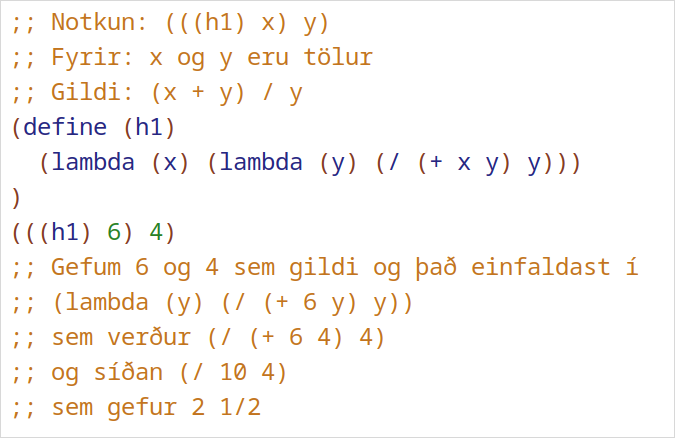
\includegraphics[scale=0.3]{h1.png}

	Við skrifum þetta í Scheme sem \texttt{(lambda (x) (lambda (y) 
	(/ (+ x y) y)))} sem skilar þá falli sem virkar þannig
	að það tekur tvenn inntök, 
	x og y, og skilar $\frac{x + y}{y}$  

	Við getum notað fallið t.d. svona: 
	\begin{verbatim}
(define (h1)
  (lambda (x) (lambda (y) (/ (+ x y) y)))
)
(((h1) 6) 4)
	\end{verbatim}
	sem skilar 
	$2\frac{1}{2}$. 

	\begin{center}
	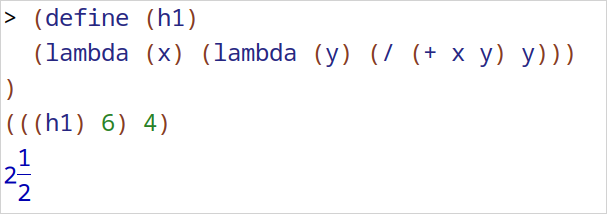
\includegraphics[scale=0.375]{64.png}
	\end{center}

	Hægt er svo að endurskrifa segðina með öðrum táknum þannig að 

	\[\lambda a.(\lambda b.(a + b) / b)\]

	Eða í Scheme:

	\begin{center}
		\texttt{(lambda (a) (lambda (b) (/ (+ a b) b)))}
	\end{center}

	\section{$((\lambda x.(\lambda y.(x + y) / y)) 3) 6$}
	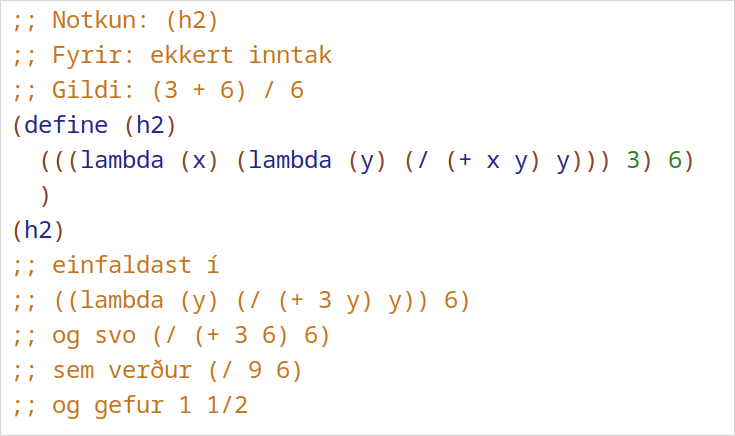
\includegraphics[scale=0.3]{h2.png}

	Í Scheme fáum við 

	\begin{verbatim}
(define (h2)
  (((lambda (x) (lambda (y) (/ (+ x y) y))) 3) 6)
  )
(h2)
	\end{verbatim}
	\vspace{-1em}
	sem skilar einfalda gildinu $1\frac{1}{2}$.

	\begin{center}
	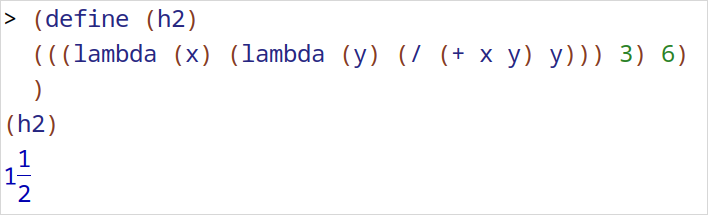
\includegraphics[scale=0.375]{36.png}
	\end{center}

	Fallið er með engar frjálsar 
	breytur og við getum endurskrifað það með öðrum táknum sem


	\[((\lambda x.(\lambda y.(x + y) / y)) 3) 6\]

	Eða í Scheme:

	\begin{center}
		\texttt{(((lambda (a) (lambda (b) (/ (+ a b) b))) 3) 6)}
	\end{center}

	\newpage
	\section{$((\lambda x.(\lambda y.(x(xy))))(\lambda x.x^2)) 3$}
	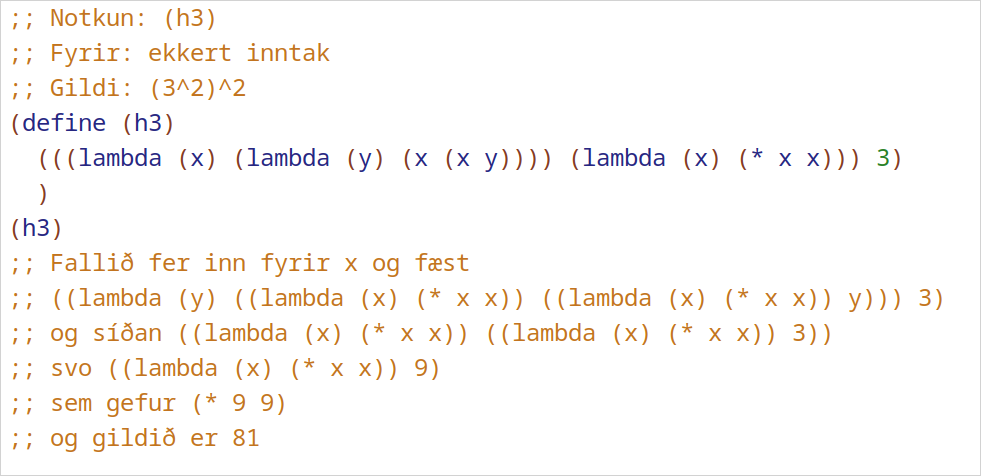
\includegraphics[scale=0.3]{h3.png}

	Þetta verður svo í Scheme: 

	\begin{center}\texttt{(((lambda (x) (lambda (y) 
	(x (x y)))) (lambda (x) (* x x))) 3)}\end{center}

	Fallið skilar einfalda gildinu 81, þar sem það skilar $(3^2)^2$

	\begin{center}
		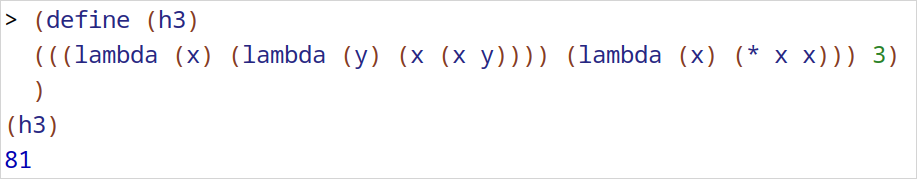
\includegraphics[scale=0.375]{81.png}
	\end{center}

	En það er með engar frjálsar breytur og 
	við getum endurskrifað það með öðrum táknum sem

	\[((\lambda a.(\lambda b.(a(a b)))) (\lambda c.c^2))3\]

	Eða í Scheme:

	\begin{center}
		\texttt{(((lambda (a) (lambda (b) (a (a b)))) (lambda (c) 
		(* c c))) 3)}
	\end{center}

\end{document}
